% Practice Test 24 — Alaska Edition
% Questions: 30 (27 MC + 3 SA)
% Generated by scripts/generate_practice_tests.py

\begin{practiceQuestion}{1-3-q15}{mc}
\begin{questionText}
Two students find $k$ from the point $(8, 20)$. Student A says $k = 2.5$. Student B says $k = 0.4$. Who is correct?
\end{questionText}
\choiceA{Student A, because $k = \frac{y}{x}$}
\choiceB{Student B, because $k = \frac{x}{y}$}
\choiceC{Both are correct, depending on which variable is independent}
\choiceD{Neither is correct}
\correctAnswer{A}
\explanation{By convention, $k = \frac{y}{x} = \frac{20}{8} = 2.5$. Student B computed $\frac{x}{y}$, which is the reciprocal — not $k$.}
\end{practiceQuestion}

\begin{practiceQuestion}{1-5-q01}{mc}
\begin{questionText}
The equation $y = 5x$ gives the cost of movie tickets. What does the point $(1, 5)$ represent?
\end{questionText}
\choiceA{$5$ movies cost $\$1$}
\choiceB{$1$ ticket costs $\$5$}
\choiceC{The total for all tickets is $\$5$}
\choiceD{You need $5$ hours to buy $1$ ticket}
\correctAnswer{B}
\explanation{The point $(1, 5)$ means $x = 1$ ticket and $y = \$5$, so one ticket costs $\$5$. This is the unit rate.}
\end{practiceQuestion}

\begin{practiceQuestion}{1-6-q05}{mc}
\begin{questionText}
A printer prints $120$ pages in $8$ minutes. How long will it take to print $450$ pages?
\end{questionText}
\choiceA{$25$ min}
\choiceB{$28$ min}
\choiceC{$30$ min}
\choiceD{$36$ min}
\correctAnswer{C}
\explanation{Rate: $120 \div 8 = 15$ pages/min. Time for $450$: $450 \div 15 = 30$ min.}
\end{practiceQuestion}

\begin{practiceQuestion}{2-2-q06}{mc}
\begin{questionText}
In a bag of $150$ marbles, $60$ are blue. What percent of the marbles are blue?
\end{questionText}
\choiceA{$25\%$}
\choiceB{$30\%$}
\choiceC{$35\%$}
\choiceD{$40\%$}
\correctAnswer{D}
\explanation{$\frac{60}{150} = \frac{p}{100}$. Cross-multiply: $150p = 6000$. Divide: $p = 40\%$.}
\end{practiceQuestion}

\begin{practiceQuestion}{2-5-q09}{mc}
\begin{questionText}
A hair stylist charges $\$55$ for a haircut. The customer leaves a $20\%$ tip. What is the total the customer pays?
\end{questionText}
\choiceA{$\$11.00$}
\choiceB{$\$60.50$}
\choiceC{$\$66.00$}
\choiceD{$\$75.00$}
\correctAnswer{C}
\explanation{$55 \times 1.20 = \$66.00$.}
\end{practiceQuestion}

\begin{practiceQuestion}{3-1-q07}{mc}
\begin{questionText}
A diver is at $-15$ feet (below sea level). What does $|-15|$ represent in this context?
\end{questionText}
\choiceA{The diver is $15$ feet above sea level}
\choiceB{The diver's distance from sea level is $15$ feet}
\choiceC{The diver moves $15$ feet deeper}
\choiceD{The diver returns to sea level}
\correctAnswer{B}
\explanation{The absolute value $|-15| = 15$ represents the distance from zero (sea level), regardless of direction.}
\end{practiceQuestion}

\begin{practiceQuestion}{3-2-q11}{mc}
\begin{questionText}
You owe $\$25$ and borrow $\$10$ more. Which expression represents your total debt?
\end{questionText}
\choiceA{$25 + 10 = 35$}
\choiceB{$(-25) + 10 = -15$}
\choiceC{$(-25) + (-10) = -35$}
\choiceD{$25 - 10 = 15$}
\correctAnswer{C}
\explanation{Owing money is negative. You owe $\$25$ ($-25$) and borrow $\$10$ more ($-10$): $(-25) + (-10) = -35$.}
\end{practiceQuestion}

\begin{practiceQuestion}{3-3-q30}{gsa}
\begin{questionText}
The diagram shows two floors in a building. The parking garage is at level $-3$ and the rooftop is at level $5$.

\begin{center}
\begin{tikzpicture}
  \draw[thick] (0,-3.5) -- (0,5.5);
  \foreach \y in {-3,...,5} {
    \draw (-0.3,\y) -- (0.3,\y);
    \node[right=6pt] at (0,\y) {Level $\y$};
  }
  \fill[funRed] (0,-3) circle (4pt) node[left=10pt] {Garage};
  \fill[funBlue] (0,5) circle (4pt) node[left=10pt] {Rooftop};
  \draw[dashed,gray] (-0.5,0) -- (0.5,0);
  \node[left=20pt] at (0,0) {Ground};
\end{tikzpicture}
\end{center}

How many levels apart are the garage and the rooftop?
\end{questionText}
\correctAnswer{$8$ levels}
\explanation{$|5 - (-3)| = |5 + 3| = |8| = 8$ levels.}
\end{practiceQuestion}

\begin{practiceQuestion}{3-10-q07}{mc}
\begin{questionText}
A checking account has $\$320.45$. Three checks are written for $\$85.20$, $\$142.75$, and $\$98.50$. What is the new balance?
\end{questionText}
\choiceA{$\$-6.00$}
\choiceB{$\$6.00$}
\choiceC{$\$646.90$}
\choiceD{$-\$646.90$}
\correctAnswer{A}
\explanation{$320.45 - 85.20 - 142.75 - 98.50 = 320.45 - 326.45 = -6.00$. Overdrawn by $\$6.00$.}
\end{practiceQuestion}

\begin{practiceQuestion}{4-1-q29}{gsa}
\begin{questionText}
A parking garage charges the rates shown in the sign below.

\begin{center}
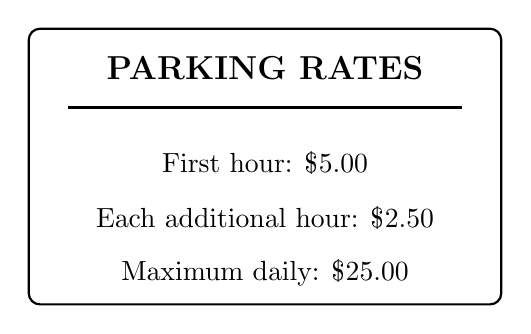
\begin{tikzpicture}
  \draw[thick, rounded corners] (0,0) rectangle (6,3.5);
  \node[font=\bfseries\large] at (3,3) {PARKING RATES};
  \draw[thick] (0.5,2.5) -- (5.5,2.5);
  \node[align=left] at (3,1.8) {First hour: \$5.00};
  \node[align=left] at (3,1.1) {Each additional hour: \$2.50};
  \node[align=left] at (3,0.4) {Maximum daily: \$25.00};
\end{tikzpicture}
\end{center}

Write an expression for the cost of parking for $h$ hours (where $h \geq 1$), and find the cost of parking for $6$ hours.
\end{questionText}
\correctAnswer{$2.50h + 2.50$ (or $5 + 2.50(h-1)$); $\$17.50$}
\explanation{The first hour costs $\$5.00$. Each additional hour costs $\$2.50$, so for $h$ hours the additional hours cost $2.50(h - 1)$. Total: $5 + 2.50(h - 1) = 5 + 2.50h - 2.50 = 2.50h + 2.50$. For $h = 6$: $2.50(6) + 2.50 = 15 + 2.50 = \$17.50$.}
\end{practiceQuestion}

\begin{practiceQuestion}{5-2-q10}{mc}
\begin{questionText}
Which equation has the solution $x = 5$?
\end{questionText}
\choiceA{$4x + 3 = 18$}
\choiceB{$4x + 3 = 23$}
\choiceC{$4x - 3 = 23$}
\choiceD{$4x - 5 = 25$}
\correctAnswer{B}
\explanation{Substitute $x = 5$: $4(5) + 3 = 20 + 3 = 23$. So $4x + 3 = 23$ is correct.}
\end{practiceQuestion}

\begin{practiceQuestion}{5-3-q01}{mc}
\begin{questionText}
Solve $2(x + 6) = 20$.
\end{questionText}
\choiceA{$x = 4$}
\choiceB{$x = 7$}
\choiceC{$x = 10$}
\choiceD{$x = 14$}
\correctAnswer{A}
\explanation{Divide both sides by $2$: $x + 6 = 10$. Subtract $6$: $x = 4$. Check: $2(4 + 6) = 2(10) = 20$ \checkmark.}
\end{practiceQuestion}

\begin{practiceQuestion}{5-4-q13}{mc}
\begin{questionText}
A shirt is on sale for $\dfrac{2}{3}$ of its original price. After using a $\$5$ coupon, you pay $\$15$. What equation finds the original price $p$?
\end{questionText}
\choiceA{$\dfrac{2}{3}p + 5 = 15$}
\choiceB{$p - \dfrac{2}{3} - 5 = 15$}
\choiceC{$\dfrac{2}{3}p - 5 = 15$}
\choiceD{$\dfrac{2}{3}(p - 5) = 15$}
\correctAnswer{C}
\explanation{Sale price is $\frac{2}{3}p$. After the $\$5$ coupon: $\frac{2}{3}p - 5 = 15$.}
\end{practiceQuestion}

\begin{practiceQuestion}{5-5-q02}{mc}
\begin{questionText}
Solve $-3n + 6 \leq 0$.
\end{questionText}
\choiceA{$n \leq 2$}
\choiceB{$n \leq -2$}
\choiceC{$n \geq 2$}
\choiceD{$n \geq -2$}
\correctAnswer{C}
\explanation{Subtract $6$: $-3n \leq -6$. Divide by $-3$ and flip the sign: $n \geq 2$.}
\end{practiceQuestion}

\begin{practiceQuestion}{5-6-q16}{mc}
\begin{questionText}
Solve $\dfrac{x}{2} - 3 > 1$ and describe the graph.
\end{questionText}
\choiceA{Open circle at $8$, shade right}
\choiceB{Closed circle at $8$, shade right}
\choiceC{Open circle at $4$, shade right}
\choiceD{Open circle at $8$, shade left}
\correctAnswer{A}
\explanation{Add $3$: $\frac{x}{2} > 4$. Multiply by $2$: $x > 8$. Open circle at $8$, shade right.}
\end{practiceQuestion}

\begin{practiceQuestion}{6-2-q10}{mc}
\begin{questionText}
A blueprint uses $1$ in $= 12$ ft. You redraw at $1$ in $= 4$ ft. A door that is $0.5$ in wide on the original becomes how wide?
\end{questionText}
\choiceA{$0.5$ in}
\choiceB{$1$ in}
\choiceC{$1.5$ in}
\choiceD{$3$ in}
\correctAnswer{C}
\explanation{Scale ratio: $\frac{12}{4} = 3$. New width: $0.5 \times 3 = 1.5$ in.}
\end{practiceQuestion}

\begin{practiceQuestion}{6-3-q07}{mc}
\begin{questionText}
A rectangle must have a perimeter of $24$ cm. How many different rectangles can satisfy this condition?
\end{questionText}
\choiceA{None}
\choiceB{Exactly one}
\choiceC{Exactly two}
\choiceD{More than one}
\correctAnswer{D}
\explanation{The sides must add to $12$. Many dimension pairs work: $1 \times 11$, $2 \times 10$, $3 \times 9$, etc. Perimeter alone does not fix the rectangle.}
\end{practiceQuestion}

\begin{practiceQuestion}{6-4-q04}{mc}
\begin{questionText}
Two sides of a triangle are $9$ cm and $12$ cm with an included angle of $60°$. What type of condition is this?
\end{questionText}
\choiceA{SSS}
\choiceB{SAS}
\choiceC{ASA}
\choiceD{AAA}
\correctAnswer{B}
\explanation{Two sides and the angle between them is the SAS (Side-Angle-Side) condition.}
\end{practiceQuestion}

\begin{practiceQuestion}{6-5-q09}{mc}
\begin{questionText}
You cut a cone with a vertical slice through its apex (tip). What shape is the cross-section?
\end{questionText}
\choiceA{Circle}
\choiceB{Triangle}
\choiceC{Rectangle}
\choiceD{Semicircle}
\correctAnswer{B}
\explanation{A vertical cut through the apex of a cone produces a triangle (specifically an isosceles triangle).}
\end{practiceQuestion}

\begin{practiceQuestion}{7-3-q15}{mc}
\begin{questionText}
A quarter-circle has a radius of $8$ cm. What is its area? Use $\pi \approx 3.14$.
\end{questionText}
\choiceA{$200.96$ cm$^2$}
\choiceB{$100.48$ cm$^2$}
\choiceC{$50.24$ cm$^2$}
\choiceD{$25.12$ cm$^2$}
\correctAnswer{C}
\explanation{Full circle area $= \pi r^2 = 3.14 \times 64 = 200.96$ cm$^2$. Quarter circle $= 200.96 \div 4 = 50.24$ cm$^2$.}
\end{practiceQuestion}

\begin{practiceQuestion}{7-4-q18}{mc}
\begin{questionText}
A pentagon can be divided into a rectangle $6$ cm by $4$ cm and a triangle with base $6$ cm and height $2$ cm. What is the total area?
\end{questionText}
\choiceA{$24$ cm$^2$}
\choiceB{$30$ cm$^2$}
\choiceC{$36$ cm$^2$}
\choiceD{$48$ cm$^2$}
\correctAnswer{B}
\explanation{Rectangle: $6 \times 4 = 24$ cm$^2$. Triangle: $\frac{1}{2} \times 6 \times 2 = 6$ cm$^2$. Total: $24 + 6 = 30$ cm$^2$.}
\end{practiceQuestion}

\begin{practiceQuestion}{7-5-q01}{mc}
\begin{questionText}
What is the surface area of a cube with side length $4$ cm?
\end{questionText}
\choiceA{$16$ cm$^2$}
\choiceB{$64$ cm$^2$}
\choiceC{$96$ cm$^2$}
\choiceD{$24$ cm$^2$}
\correctAnswer{C}
\explanation{A cube has $6$ faces. $SA = 6s^2 = 6 \times 16 = 96$ cm$^2$.}
\end{practiceQuestion}

\begin{practiceQuestion}{7-6-q10}{mc}
\begin{questionText}
A rectangular prism has a base area of $24$ cm$^2$ and a height of $7$ cm. What is its volume?
\end{questionText}
\choiceA{$31$ cm$^3$}
\choiceB{$168$ cm$^3$}
\choiceC{$336$ cm$^3$}
\choiceD{$17$ cm$^3$}
\correctAnswer{B}
\explanation{$V = Bh = 24 \times 7 = 168$ cm$^3$.}
\end{practiceQuestion}

\begin{practiceQuestion}{8-1-q02}{mc}
\begin{questionText}
A researcher wants to know the average height of seventh graders in a state. She measures the heights of $100$ seventh graders from different schools. What is the sample?
\end{questionText}
\choiceA{All seventh graders in the state}
\choiceB{All students in the schools she visited}
\choiceC{The $100$ seventh graders she measured}
\choiceD{The tallest seventh graders}
\correctAnswer{C}
\explanation{The sample is the smaller group chosen from the population — the $100$ students measured.}
\end{practiceQuestion}

\begin{practiceQuestion}{8-3-q26}{gmc}
\begin{questionText}
The box plots below compare test scores for Class A and Class B.

\begin{center}
\begin{tikzpicture}[scale=0.1]
  \draw[thick,->] (49,0) -- (101,0);
  \foreach \x in {50,55,...,100} {
    \draw (\x,0.5) -- (\x,-0.5);
    \node[below,font=\small] at (\x,-0.5) {$\x$};
  }
  % Class A: min=60, Q1=70, med=78, Q3=85, max=95
  \draw[thick] (60,6) -- (95,6);
  \draw[thick,fill=funBlue!30] (70,4) rectangle (85,8);
  \draw[very thick,funBlue] (78,4) -- (78,8);
  \draw[thick] (60,4) -- (60,8);
  \draw[thick] (95,4) -- (95,8);
  \node[right,font=\small] at (96,6) {Class A};
  % Class B: min=50, Q1=58, med=65, Q3=72, max=80
  \draw[thick] (50,14) -- (80,14);
  \draw[thick,fill=funGreen!30] (58,12) rectangle (72,16);
  \draw[very thick,funGreen] (65,12) -- (65,16);
  \draw[thick] (50,12) -- (50,16);
  \draw[thick] (80,12) -- (80,16);
  \node[right,font=\small] at (81,14) {Class B};
\end{tikzpicture}
\end{center}

Which statement is best supported by the box plots?
\end{questionText}
\choiceA{Class B scored higher than Class A}
\choiceB{Class A has a higher median and a larger IQR}
\choiceC{Class A has a higher median and both classes have the same IQR}
\choiceD{Class A and Class B overlap, but Class A's median is higher}
\correctAnswer{D}
\explanation{Class A median $= 78$, Class B median $= 65$. Class A's range ($60$--$95$) overlaps with Class B's range ($50$--$80$), but Class A is higher overall.}
\end{practiceQuestion}

\begin{practiceQuestion}{8-4-q16}{mc}
\begin{questionText}
Group A: $\{60, 65, 70, 75, 80\}$. Group B: $\{40, 55, 70, 85, 100\}$. Both have a mean of $70$. Which group is more variable?
\end{questionText}
\choiceA{Group A}
\choiceB{Group B}
\choiceC{They are equally variable}
\choiceD{Cannot be determined}
\correctAnswer{B}
\explanation{Group A range $= 20$, Group B range $= 60$. Group B's data is far more spread out.}
\end{practiceQuestion}

\begin{practiceQuestion}{8-7-q27}{gmc}
\begin{questionText}
The double bar graph shows the number of goals scored by two soccer teams over four games.

\begin{center}
\begin{tikzpicture}[scale=0.55]
  \draw[thick,->] (0,0) -- (0,6) node[above]{\small Goals};
  \draw[thick,->] (0,0) -- (10,0);
  % Game 1
  \fill[funBlue!70] (0.5,0) rectangle (1.2,3);
  \fill[funGreen!70] (1.3,0) rectangle (2.0,2);
  \node[below,font=\tiny] at (1.25,0) {G1};
  % Game 2
  \fill[funBlue!70] (2.5,0) rectangle (3.2,4);
  \fill[funGreen!70] (3.3,0) rectangle (4.0,5);
  \node[below,font=\tiny] at (3.25,0) {G2};
  % Game 3
  \fill[funBlue!70] (4.5,0) rectangle (5.2,2);
  \fill[funGreen!70] (5.3,0) rectangle (6.0,3);
  \node[below,font=\tiny] at (5.25,0) {G3};
  % Game 4
  \fill[funBlue!70] (6.5,0) rectangle (7.2,5);
  \fill[funGreen!70] (7.3,0) rectangle (8.0,4);
  \node[below,font=\tiny] at (7.25,0) {G4};
  \foreach \y in {1,...,5} { \draw (-0.1,\y) -- (0.1,\y); \node[left,font=\tiny] at (0,\y) {$\y$}; }
  % legend
  \fill[funBlue!70] (8.5,5) rectangle (9,5.3);
  \node[right,font=\tiny] at (9,5.15) {Team A};
  \fill[funGreen!70] (8.5,4.3) rectangle (9,4.6);
  \node[right,font=\tiny] at (9,4.45) {Team B};
\end{tikzpicture}
\end{center}

Which team scored more total goals?
\end{questionText}
\choiceA{Team A with $14$ goals}
\choiceB{Team B with $14$ goals}
\choiceC{They tied with $14$ goals each}
\choiceD{Team A with $12$ goals}
\correctAnswer{C}
\explanation{Team A: $3+4+2+5 = 14$. Team B: $2+5+3+4 = 14$. They tied.}
\end{practiceQuestion}

\begin{practiceQuestion}{9-4-q09}{mc}
\begin{questionText}
A teacher predicted that a spinner would land on red $\frac{1}{4}$ of the time. After $80$ spins, red appeared $25$ times. How do the observed and predicted results compare?
\end{questionText}
\choiceA{They are very different — the model is wrong}
\choiceB{The observed ($\frac{25}{80} = 0.3125$) is close to the predicted ($0.25$)}
\choiceC{The observed result is exactly equal to the predicted result}
\choiceD{The predicted probability is higher than the observed}
\correctAnswer{B}
\explanation{Predicted: $\frac{1}{4} = 0.25$. Observed: $\frac{25}{80} = 0.3125$. They are close, which supports the model.}
\end{practiceQuestion}

\begin{practiceQuestion}{9-6-q18}{mc}
\begin{questionText}
Three coins are flipped. What is the probability of getting NO heads (all tails)?
\end{questionText}
\choiceA{$\frac{1}{2}$}
\choiceB{$\frac{1}{4}$}
\choiceC{$\frac{1}{8}$}
\choiceD{$\frac{3}{8}$}
\correctAnswer{C}
\explanation{Only one outcome out of $8$ is all tails (TTT). $P = \frac{1}{8}$.}
\end{practiceQuestion}

\begin{practiceQuestion}{9-7-q24}{sa}
\begin{questionText}
Describe how to use a standard die to simulate a $\frac{1}{3}$ probability event.
\end{questionText}
\correctAnswer{Roll the die; let $1$ and $2$ represent the event (or any $2$ numbers out of $6$)}
\explanation{Choose $2$ of the $6$ faces to represent the event. $P = \frac{2}{6} = \frac{1}{3}$.}
\end{practiceQuestion}
